%In this section we discuss how the Provenance Data Model interacts with
%classes and attributes from other VO data models (especially DatasetDM).
%(e.g. DatasetDM, SpectralDM (share some same classes), SimDM) 
%and how provenance information can be stored.

The Provenance Data Model can be applied without making any links to other 
IVOA data model classes. For example when the data is not yet published, provenance information
can be stored already, but a DatasetDM-description for the data may not yet exist.
But if there are data models implemented for the datasets, then it is 
very useful to connect the classes and attributes of the other data models with Provenance classes and attributes (if applicable), which we are going to discuss in this Section. These links help to avoid 
unnecessary repetitions in the metadata of datsets, and also offer the possibility 
to derive some basic provenance information from existing data model classes automatically.


\subsection{Links with Dataset/Obscore Model}
Entities and their descriptions in the Provenance Data Model 
are tightly linked to the \class{DataSet}-class in the DatasetDM/ObsCore Data Model, as well as to 
InputDataset and OutputDataSet in the Simulation Data Model \citep[SimDM,][]{std:SimDM}.
Table \ref{tab:datasetmapping} maps classes and attributes from the Dataset Data Model 
to concepts in the Provenance Data Model.


%\begin{figure}[h]
%\centering
%\includegraphics[width=\textwidth]{../datamodel-diagrams/images/classes-relations-dms}
%\caption{Links between Agent and Party, Entity and Dataset.}
%\label{fig:class-relations-dm}
%\end{figure}
% --> a similar figure is already given in the sections on entity and agent.

\begin{table}[h]
\small
\tymax  0.5\textwidth
\begin{tabulary}{1.0\textwidth}{@{}lLp{4cm}@{}}
\toprule
\head{Dataset DM} & \head{Provenance DM} & \head{Comment}\\
\midrule
DataID.title         & Entity.name                & title of the dataset\\
DataID.collection    & HadMember.collectionId     & link to the collection to which the dataset belongs\\
DataID.creator       & Agent.name                 & name of agent\\
DataID.creatorDID    & alternative to Entity.id   & id for the dataset given by the creator, could be used if no PublisherDID exists (yet)\\
DataID.ObservationID & WasGeneratedBy.activityId  & identifier to everything describing the observation\\
DataID.date          & WasGeneratedBy.time        & date and time when the dataset was completely created\\
Curation.PublisherDID  & Entity.id                & unique identifier for the dataset assigned by the publisher\\
Curation.PublisherID   & Agent.id                 & link to the publisher, i.e. to an Agent with role=``publisher''\\
Curation.Publisher     & Agent.name               & name of the publisher\\
Curation.Date          & Entity.releaseDate       & release date of the dataset\\
Curation.Version       & Entity.version           & version of the dataset\\
Curation.Rights        & Entity.rights            & access rights to the dataset; one of [...]\\
Curation.Reference     & Entity.link              & link to publication\\
Curation.Contact       & Agent                    & link to Agent with role contact\\
DataProductType  & EntityDescription.dataproduct\_type & type of a dataproduct/entity\\
DataProductSubType & EntityDescription.dataproduct\_subtype & subtype of a dataproduct/entity\\
ObsDataset.calibLevel  & EntityDescription.level & (output) calibration level, integer between 0 and 3\\\hline
\bottomrule
\end{tabulary}
\caption{Mapping between attributes from classes of the Dataset Metadata Model to classes in ProvenanceDM.}
\label{tab:datasetmapping}
\end{table}



\begin{figure}[h]
\centering
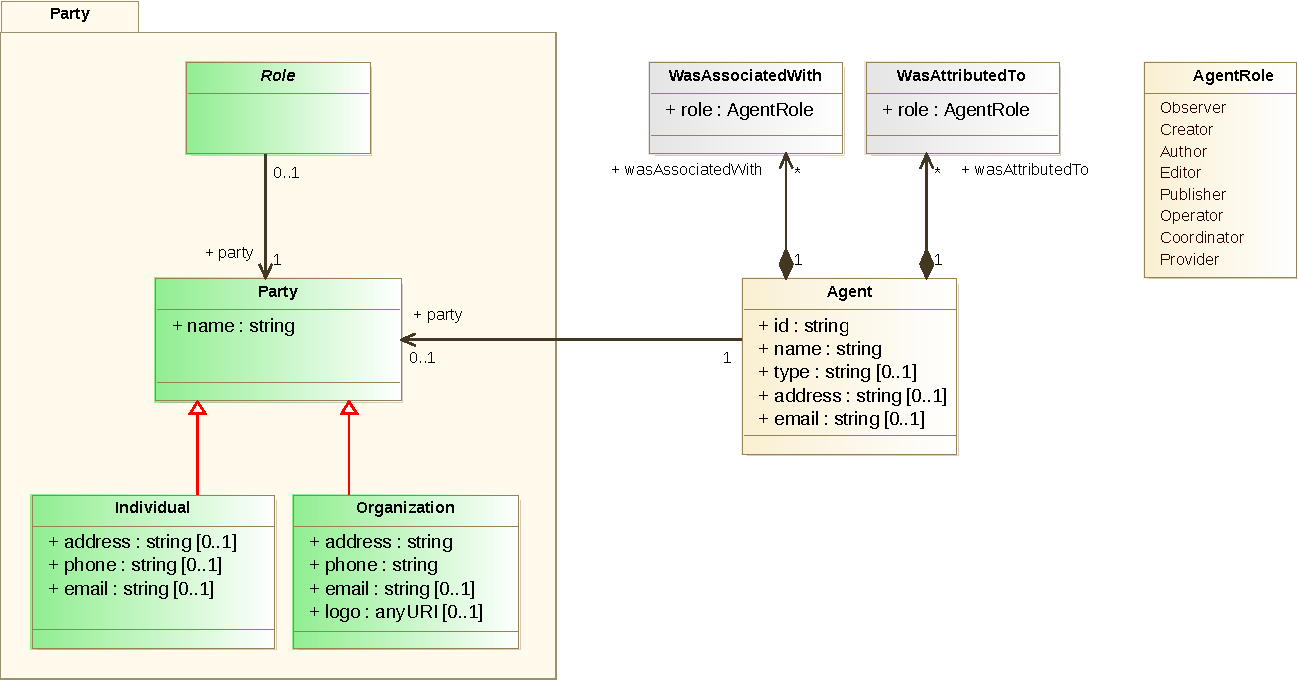
\includegraphics[width=\textwidth]{../datamodel-diagrams/images/agent-relations.pdf}
\caption{The relations between the \class{Agent} class within the Provenance Data Model 
(grey and yellow classes) with classes from the Dataset Metadata Model, party package (green).}
\label{fig:agent-relations}
\end{figure}

The \class{Agent} class, which is used for defining responsible persons and 
organizations in ProvenanceDM, is very similar to the \class{Party} class in the Dataset Metadata Model (and in SimDM). Its details are depicted in Figure~\ref{fig:agent-relations}.
The main difference between \class{Agent} and \class{Party} is that \class{Individual} and \class{Person} are subclasses in DatasetDM, whereas we just use the same class \emph{Agent} for both and distinguish between them using the \emph{Agent.type} attribute (which can have the value ``Individual'' or ``Organization'').


We imagine that services implementing both data models, \class{Dataset} and \class{ProvenanceDM} may use just \emph{one} class: either \class{Agent} or \class{Party}, enriched with all the necessary (project-specific) attributes. Note that for Provenance queries using a ProvTAP service and for W3C compatible serializations, the name \class{Agent} for the responsible individuals/organizations is required.



\subsection{Links with Simulation Data Model}
In SimDM one also encounters a normalization similar to our split-up of descriptions from 
actual data instances and executions of processes: the SimDM class ``experiment'' 
is a type of \class{Activity} and its general, reusable description is called a ``protocol'',
which can be considered as a type of this model's \class{ActivityDescription}. 
More direct mappings between classes and attributes of both models are given in Table~\ref{tab:simdmmapping}.

\begin{table}[h]
\small
\tymax  0.5\textwidth
\begin{tabulary}{1.0\textwidth}{@{}lLp{4cm}@{}}
\toprule
\head{Simulation DM} & \head{Provenance DM} & \head{Comment}\\
\midrule
Experiment      & Activity               & \\
Experiment.name & Activity.name         & human readable name; name attribute in SimDM is inherited from Resource-class\\
Experiment.executionTime  & Activity.endTime & end time of the execution of an experiment/activity \\
Experiment.protocol & Activity.activityDescription & reference to the protocol or description class \\
Protocol        & ActivityDescription    & \\
Protocol.name   & ActivityDescription.name  & human readable name\\
Protocol.referenceURL & ActivityDescription.doculink & reference to a webpage describing it\\
% add Protocol.code, Protocol.version?
ParameterSetting     & Parameter              & value of an (input) parameter\\
InputParameter       & ParameterDescription              & description of an (input) parameter\\
Party           & Agent                 & responsible person or organization\\
Party.name      & Agent.name & name of the agent \\
Contact         & WasAssociatedWith & \\
Contact.role    & WasAssociatedWith.role & role which the agent/party had for a certain experiment (activity); SimDM roles contain: \texttt{owner}, \texttt{creator}, \texttt{publisher}, \texttt{contributor}\\
Contact.party    & WasAssociatedWith.agent & reference to the agent/party \\
DataObject     & Entity        & a dataset, which can be/refer to a collection\\

\bottomrule
\end{tabulary}
\caption{Mapping between classes and attributes from SimDM to classes/attributes in ProvenanceDM.}
\label{tab:simdmmapping}
\end{table}




\subsection{Further links to data models}
More similarities and links to other data models will be detailed in future 
versions of this working draft.
